\documentclass[12pt]{article}

% Packages for formatting
\usepackage{geometry} % 1-inch margins
\geometry{a4paper, margin=1in}
\usepackage{times} % Times New Roman font
\usepackage{setspace} % For double spacing
\usepackage{csquotes}       % For proper quotation formatting \enquote{}
\usepackage{fancyhdr} % For headers and footers
\usepackage{titlesec} % For section numbering
\usepackage{booktabs} % For professional-looking tables
\usepackage{bookmark}
\usepackage{float}
\usepackage[polish,spanish,english]{babel}
\hypersetup{
    colorlinks=true,
    linkcolor=black,
    urlcolor=black,
    citecolor=black
}
\usepackage{graphicx}
\graphicspath{ {./figures/} }
\usepackage[style=apa, backend=biber, language=english]{biblatex} % APA 7th edition references
\usepackage[T1]{fontenc}
\usepackage{caption}
\captionsetup[table]{font=small, labelsep= period, labelfont=bf, width=0.8\textwidth}
\captionsetup[figure]{font=small, labelsep= period, labelfont=bf, width=0.8\textwidth} 
% Options: tiny, scriptsize, footnotesize, small, normalsize, large, Large, etc.
\usepackage{subcaption}

\addbibresource{TFM.bib} % Reference file

% Set double spacing
\doublespacing

% Indent paragraphs by 0.5 inch
\setlength{\parindent}{0.5in}

% Page numbering setup
\pagestyle{fancy}
\fancyhf{}
\rfoot{\thepage} % Page number in the bottom-right corner
\renewcommand{\headrulewidth}{0pt} % Remove the header rule

% Section formatting
\titleformat{\section}[block]{\normalfont\Large\bfseries}{\thesection.}{0.5em}{}

\begin{document}
\pagenumbering{roman}
\section*{Abstract}
This project investigates to what extent morphological inflection can be automatically distinguished from derivation based solely on word forms. The debate on inflection and derivation remains highly contentious in linguistic literature, with some viewing them as fundamentally similar or existing on a gradient, while others argue for a clear distinction. Despite extensive theoretical discussions, empirical evidence remains limited. One proposed distinction is semantic regularity: inflection is expected to be stable in its syntactic and semantic effects across lexemes (e.g., cinema is to cinemas as cat is to cats), whereas derivation is less so (e.g., delegation is not to delegate as election is to elect). However, this criterion has yet to be systematically tested large scale cross-linguistically. 
Building on previous work (e.g., \textcite{bonami2018InflectionVsDerivation}; \textcite{rosa2019AttemptingSeparateInflection}), this project uses distributional semantics and word embeddings to assess semantic regularity as a potential proxy for differentiating inflection and derivation. It focuses on two morphologically rich languages, Spanish and Polish. Additionally, the project examines differences in semantic regularity also among various types of inflection, such as case, number, gender, and person.

\section*{Keywords}
morphology, inflection, derivation, distributional semantics

\newpage
\tableofcontents % índice
\newpage

\pagenumbering{arabic}

\newpage
\section{Introduction}

% The distinction between morphological inflection and morphological derivation is still an unresolved theoretical question. In order to tell them apart, authors provide many different criteria (see for instance \textcite{booij2006InflectionDerivation}, \textcite{aronoff2011WhatMorphology}, \textcite{booij2012GrammarWordsIntroduction}, \textcite{haspelmath2013UnderstandingMorphology}, \textcite{stump2005WordFormationInflectionalMorphology} or \textcite{stump2017Inflection}, among many others). Some authors are of the opinion that they are essentially the same thing \parencite{haspelmath2024InflectionDerivationTraditional} or at least that they exist on different ends of a scale or gradient (see \textcite{bybee1985MorphologyStudyRelation} or \textcite{stekauer2015DelimitationDerivationInflection}).

% However, all authors provide hand-picked examples to support their arguments and not a single quantitative study had been done before until recently. Thanks to the widespread use of distributional vector spaces...

% The purpose of this project is to explore the inflection-derivation gradient using the semantic regularity criterion as a proxy. In order to automatically test whether this it holds or not, we need to make use of the distributional hypothesis and word vectors.

% To further explain this criterium it is also said that derivation creates new lexemes whereas inflection creates wordforms (WHAT IS A WORDFORM?) of the same lexeme, both generally using affixes. A lexeme is an abstract word that represents wordforms, that is wordforms such as \textit{eats}, \textit{ate}, \textit{eaten} all relate to a single abstract representation \textsc{eat} (written by convention in small capital letters). In other words, derivation is a lexicon enriching morphological process whereas inflection is a cell filling process.

\section{Background and rationale}

\subsection{Inflection and derivation}
Usually, a distinction between inflection and derivation is drawn. In introductory morphology books they are presented as different processes (see for instance \textcite{aronoff2011WhatMorphology, booij2012GrammarWordsIntroduction,haspelmath2013UnderstandingMorphology} or academic literature like \textcite{booij2006InflectionDerivation,stump2005WordFormationInflectionalMorphology,stump2017Inflection}). These authors and many others provide many different criteria in order to draw a boundary between both morphological processes such as: \enquote{inflection is relevant to the syntax while derivation is not}, \enquote{inflection does not change the part of speech of the base while derivation may change it} or \enquote{derivation expresses a new meaning different from the base while inflection does not}. These criteria are just a small sample of all of the them that are usually provided. % tabla con criterios tipo Bonami?

However, there have been authors that have challenged this sharp boundary view directly posing that we should not make a distinction between them \parencite{haspelmath2024InflectionDerivationTraditional} or that there is at best a continuum or gradient in which (canonical/prototypical) inflection and derivation stand on opposite sides \parencite{bybee1985MorphologyStudyRelation, stekauer2015DelimitationDerivationInflection}. Even \textcite{haspelmath2013UnderstandingMorphology} argue that if all criteria are given the same importance then a continuum is the best explanation, since we cannot draw a sharp boundary between both processes. In fact, the same authors that provide long lists of criteria also acknowledge that exceptions exist and that some inflectional processes appear derivational and some derivational processes appear inflectional. \textcite{booij2006InflectionDerivation} also draws a distinction between two different inflectional processes, inherent (not required by syntax, but a semantic choice like the use of a plural form or infinitives and participles) and contextual (required by syntax, such as verb-subject agreement or a case choice in nouns). The author argues that inherent inflection is halfway between derivation and contextual inflection, since inherent inflection also may change the part of speech of a word.

\subsection{Related studies}
Despite extensive literature on inflection and derivation, there have not been many empirical quantitative studies trying to shed light on this theoretical question until relatively recently. Thanks to computational advancements in distributional semantics (see \autoref{distributional-semantics}) some studies have tried to separate both processes using one of the commonly proposed criteria, the semantic regularity criterion. This criterion states that \enquote{Inflection is semantically more regular than derivation.} \parencite{stump2005WordFormationInflectionalMorphology}. Essentially, it says that derived lexemes stray further from the meaning of the base than inflected ones, while in inflection the core meaning stays the same. To date and to my understanding, the studies that have examined this debate in a quantitative way are the following:

\begin{itemize}
    \item \textcite{bonami2018InflectionVsDerivation} use a Word2Vec French model in order to assess if inflection is semantically more regular than derivation (semantic regularity criterion). Using a French lexicon, they construct a triplets dataset consisting of a pivot, an inflectional comparandum and a derivational comparandum based on different frequency measures. In their experiment, they measure shifts in meaning, for that they measure vector offset variance using Euclidean distance between the inflectional comparandum and the derivational comparandum. The authors clarify that using cosine similarity gives similar results on their data. They conclude that a categorical boundary between inflection and derivation cannot be found, although inflectional relations are more stable on average.
    \item \textcite{rosa2019AttemptingSeparateInflection} use a FastText Czech model (although they puposefully ignore words that do not appear in the model) to automatically separate inflection and derivation using a different criterion, the lexical meaning change criterion. They aim to determine if two morphologically related words belong to the same inflectional paradigm or are linked by derivation. Using a Czech database of word formation relations they measure string similarity (Jaro-Winkler edit distance) and cosine similarity. They find that inflectional forms are more similar to each other than derivational forms and that some derivational processess behave like inflection and vice versa, supporting the idea of a continuous scale and no strict boundary.
    \item \textcite{haley2024CorpusbasedMeasuresDiscriminate} conducted the most complete of all three studies in quantity of measures (4) and languages (26). Like the previous study, they also used FastText models for all of the languages. The authors computed four measures, two based on the orthographic form and two on the distributional characteristics, to predict whether a given construction is inflectional or derivational using UniMorph data and two types of machine learning models. Their results also indicate that there is no strict boundary between inflection and derivation, but that they belong to a gradient.
\end{itemize}

% more on the related studies

\subsection{Distributional semantics} \label{distributional-semantics}
In order to explore the semantic regularity criterion we need to be able to capture the meaning of the words and nowadays, in order to capture it, we make use of distributional semantics. They are based on the distributional hypothesis which essentially states that similar words appear in similar contexts \parencite{boleda2020DistributionalSemanticsLinguistic}. Distributional semantics represent the meaning of words as vectors, that is points in a multidimensional space, and similar words will also have similar vector thus occupying a similar space. In the semantic space created by the distributional model we can see the relation between specific words looking at the geometric relations of their vectors, using either Euclidean distance (the length of the straight line between them) or, more commonly, cosine similarity (the cosine of the angle between the vectors) \parencite{boleda2020DistributionalSemanticsLinguistic,chandrasekaran2021EvolutionSemanticSimilarity}. The vectors in this context are also often called word embeddings. For the current study two different static word embedding models were used, namely \textit{Word2Vec} \parencite{mikolov2013EfficientEstimationWord}, \textit{FastText} \parencite{bojanowski2017EnrichingWordVectors} (see \autoref{methodology} for a detailed explanation of the specific models). The main difference between both is that \textit{word2Vec} operates on word level and \textit{fastText} on a subword level. This means \textit{fastText} can compute word representations for words that were not in the training data \parencite{bojanowski2017EnrichingWordVectors}. % extend this explanation
For details on the specific models used in this study see \autoref{methodology}.

\subsection{UniMorph}

UniMorph is a database that provides annotated morphological inflection tables and derivational morphology of numerous languages \parencite{batsuren2022UniMorph40Universal}.

\section{Methodology} \label{methodology}

This study explores the distinction between inflection and derivation in Polish and Spanish using two static word embedding models. The \textit{word2vec} model for Spanish was trained on the Spanish Billion Words (SBW) corpus (DESCRIBE CORPORA HERE). For Polish, the IPIPAN \textit{word2vec} model (nkjp+wiki-forms-all-300-skipg-ns) was used, which is comparable in quality to SBW. It was trained on the National Corpus of Polish (NKJP) and Wikipedia, includes all parts of speech and word forms, and produces 300-dimensional vectors using the skip-gram algorithm with negative sampling. In addition, FastText embeddings for both Spanish and Polish were applied to incorporate subword-level information.

% It is important to note that these languages were chosen out of convenience, there are many resources available, and there were not any other similar studies done on these specific languages.


\subsection{Constructing the datasets}

In order to conduct the analysis two separate datasets were constructed, one for inflection and another one for derivation, extracting the necessary data from UniMorph. For the inflection analysis, a pivot/inflection dataframe was constructed. The data was filtered to include only the following verb tenses in Spanish: Present Indicative (UniMorph tag: V;IND;PRS), Past Imperfect (UniMorph tag: V;IND;PST;IPFV) and Future Indicative (UniMorph tag: V;IND;FUT). A second filter was applied on the resulting data to remove \textit{vos} and \textit{usted} forms. \textit{Voseo} forms do not have a high occurrence and \textit{usted} forms are essentially duplicated forms since they are the same as 3rd person singular forms. This resulted in a dataframe of 148,051 rows (CHECK NUM OF ROWS) , each consisting of a base form (pivot), its inflected form (inflection), and its morphological category. In Polish the filtering included the same verb tenses: Present (UniMorph tag: V;PRS), Past (UniMorph tag:V;PST) and Future (UniMorph tag:V;FUT). The resulting dataset contains 23,615 rows. 

\begin{table}[h!]
    \centering
    \small
    \begin{tabular}{lll}
        \toprule
        \textbf{Pivot} & \textbf{Inflection} & \textbf{Category} \\ 
        \midrule
        honrar	& honro &	V;IND;PRS;1;SG \\
        honrar	& honras &	V;IND;PRS;2;SG;INFM \\
        honrar	& honra &	V;IND;PRS;3;SG \\
        honrar	& honramos &	V;IND;PRS;1;PL \\
        honrar	& honráis &	V;IND;PRS;2;PL \\
        honrar	& honran &	V;IND;PRS;3;PL \\
        \bottomrule
    \end{tabular}
    \caption{Inflections dataframe sample.}
    \label{tab:infl-sample}
\end{table}

In the derivation data, the label U (unspecified or unknown) was either fixed or removed. In Spanish there are 20 rows that contain a derivation that results in U (X:U) and 107 in Polish. On the other hand, there are even more derivations in which the pivot is tagged with U (U:X), 36 in Spanish and 253 in Polish.

In order to clean the Spanish derivations dataset a new category according to the affix was assigned to the pivot position. All the affixes that end in \textit{-ero}, \textit{-ez}, \textit{-ismo}, \textit{-í} and \textit{-illa} were changed from U (U:X) to N (N:X), since all these are noun affixes. The category was also assigned (V:X) to those that contain the affixes \textit{-ar} and \textit{-ear}. As a result 6 rows were left over and eliminated from the final dataframe because they simply contained mistakes. Fixing the category assigned to the derivation position (X:U) proved trickier. There are numerals and words that are not nouns, adjectives, adverbs or verbs (all the UniMorph categories). The latter can simply be dropped, and since numerals could be tagged as either N or ADJ, they can also be dropped. The total number of wrongly tagged rows in this case is low (36), so it will have no major influence on the results.

Regarding the fixes in the Polish data, some rows incorrectly labelled U in the derivation position were fixed looking at the affixes. The affixes \textit{-any}, \textit{-ony}, \textit{-ty}, \textit{-y}, or \textit{-ący}, \textit{-ęty} should take the label ADJ, because they are all endings that participles take. There also are some formatting issues. Some rows under the same condition contain the pivot and the derived form joined together in the pivot cell (i.e. \textit{mylićpomylić pomylić}). This was fixed as well just removing the derivation from the pivot column. Some rows that contained verbs in both columns but were not correctly labeled in the derivation form were fixed as well. Three specific rows incorrectly labeled U:U were changed to ADJ:ADJ since they contained adjectives. The rest can be removed as well as they do not contain any nouns, adjectives, adverbs or verbs.

There are more incorrectly labelled rows in the Polish data. There are many rows (163) that contain infinitives in both the pivot and the derivation column, but are incorrectly labelled U:V. In Polish, infinitives end in \textit{-ć} or \textit{-c}, so the label correction was easily done. Since almost 200 rows have been fixed, the resulting ones labeled U:X are not many (21). They also contain mistakes, such as words that are not nouns, adjectives,adverbs or verbs so they can just be dropped. Both the Spanish and Polish dataframes do not contain any row labeled with U anymore.

\subsection{Obtaining the mean similarity}

% description of the whole python process

\subsection{Subsetting the most frequent lemmas and affixes}

For this task in Spanish the 10000 most frequent lemmas in CREA was used. The verbs that appear in both datasets, UniMorph and CREA, were extracted and a subset of 1568 lemmas was obtained from a total of 6695. 

For the Polish data sgjp.pl was used. Using the site's implemented filter the 8500 most common lexemes were extracted and after filtering the verbs from that list, 1832 verbs were obtained. Afterwards that list of verbs was compared to the UniMorph data and  those that appear in both datasets were extracted resulting in 455 lemmas from a total of 844 that appear in the UniMorph data.

To create the subset of affixes, the most common affixes in the UniMorph data itself were taken.

\begin{table}[htbp]
\centering
\small
\label{tbl:affixes}
\begin{minipage}[t]{0.48\textwidth}
\centering
\subcaption*{Spanish}
\begin{tabular}{lr}
\toprule
\textbf{Affix} & \textbf{Count} \\
\midrule
-mente  & 2997 \\
-dor    & 1316 \\
-ar     & 1310 \\
-ero    & 1123 \\
-miento & 913  \\
-ico    & 870  \\
des-    & 836  \\
-ción   & 831  \\
-ear    & 676  \\
-ista   & 642  \\
-ito    & 638  \\
-ismo   & 549  \\
-ón     & 533  \\
-idad   & 499  \\
-al     & 491  \\
\bottomrule
\end{tabular}
\end{minipage}
\hfill
\begin{minipage}[t]{0.48\textwidth}
\centering
\subcaption*{Polish}
\begin{tabular}{lr}
\toprule
\textbf{Affix} & \textbf{Count} \\
\midrule
-owy   & 5804 \\
-ka    & 5487 \\
-anie  & 3421 \\
-ość  & 3287 \\
-ny    & 2414 \\
-ie    & 2161 \\
-enie  & 1669 \\
-ek    & 1521 \\
-ować  & 1517 \\
-o     & 1393 \\
-ik    & 1249 \\
-ski   & 1212 \\
-ąć   & 1158 \\
-stwo  & 770  \\
za-    & 742  \\
\bottomrule
\end{tabular}
\end{minipage}
\caption{Top 15 affixes in Spanish and Polish in UniMorph data.}
\end{table}


\begin{table}[htbp]
\centering
\label{tbl:subset-results}
\begin{minipage}[t]{0.48\textwidth}
\small
\centering
\subcaption*{Inflection}
\begin{tabular}{llc}
\toprule
\textbf{Model} & \textbf{Language} & \textbf{Mean Similarity} \\
\midrule
\textbf{FastText}  & Spanish & 0.49 \\
                   & Polish  & 0.49 \\
\textbf{Word2Vec}  & Spanish & 0.50 \\
                   & Polish  & 0.53 \\
\textbf{BERT}      & Spanish & 0.82 \\
                   & Polish  & 0.73 \\
\bottomrule
\end{tabular}
\end{minipage}
\hfill
\begin{minipage}[t]{0.48\textwidth}
\small
\centering
\subcaption*{Derivation}
\begin{tabular}{llc}
\toprule
\textbf{Model} & \textbf{Language} & \textbf{Mean Similarity} \\
\midrule
\textbf{FastText}  & Spanish & 0.51 \\
                   & Polish  & 0.54 \\
\textbf{Word2Vec}  & Spanish & 0.50 \\
                   & Polish  & 0.40 \\
\textbf{BERT}      & Spanish & 0.82 \\
                   & Polish  & 0.83 \\
\bottomrule
\end{tabular}
\end{minipage}
\caption{Mean similarity between pivot and form in inflection and derivation by model and language on the subset data.}
\end{table}

% shuffled data plot, subset data plot

\subsection{Implementing a random baseline}
In order to evaluate the effectiveness of the methodology and provide a point of comparison, a baseline was implemented. It consisted of filtering the data, that is separately filtering inflections by tense (present, past or future) and derivations by category, then each filter was shuffled 100 times while extracting the mean similarity of the whole filtered data. That is, the mean similarity was extracted 100 times by type of morphological process (inflection or derivation), tense/category, model and language. The distribution is shown in \autoref{fig:baseline}.

\begin{figure}[p]
\centering
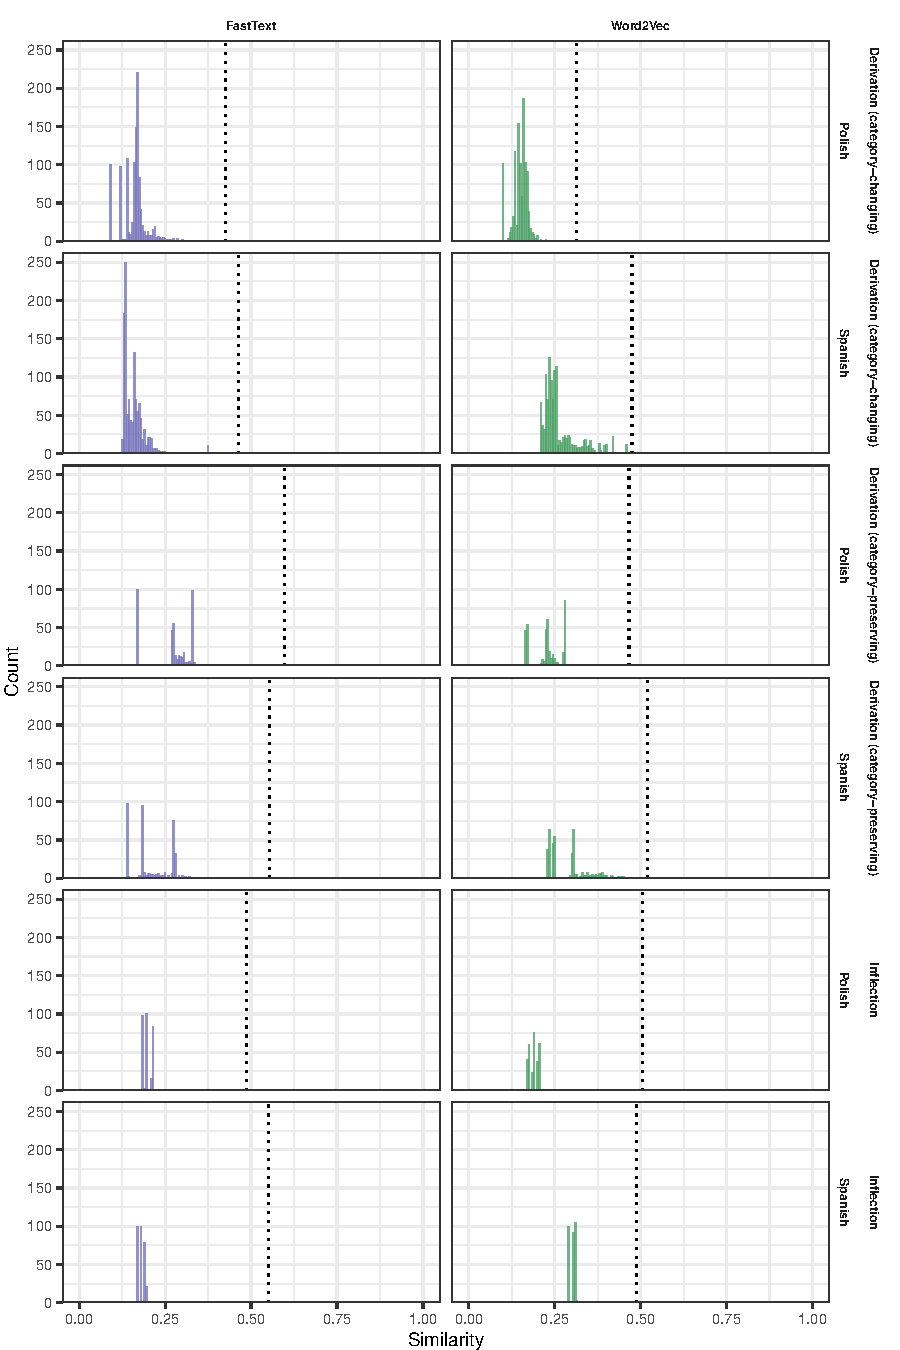
\includegraphics{fig-baseline-faceted.pdf}
\caption{Distribution of the random baseline results. The dotted line represents the mean similarity value on the clean data.}
\label{fig:baseline}
\end{figure}

\subsection{Statistical analysis}

\section{Results}

\begin{table}[ht]
\centering
\label{tbl:mean-similarity}
\begin{minipage}[t]{0.48\textwidth}
\small
\centering
\subcaption*{Inflection}
\begin{tabular}{llc}
\toprule
\textbf{Model} & \textbf{Language} & \textbf{Mean Similarity} \\
\midrule
\textbf{FastText}  & Spanish & 0.51 \\
                   & Polish  & 0.54 \\
\textbf{Word2Vec}  & Spanish & 0.50 \\
                   & Polish  & 0.40 \\
\textbf{Mult BERT} & Spanish & 0.92 \\
                   & Polish  & 0.93 \\
\bottomrule
\end{tabular}
\end{minipage}
\hfill
\begin{minipage}[t]{0.48\textwidth}
\small
\centering
\subcaption*{Derivation}
\begin{tabular}{llc}
\toprule
\textbf{Model} & \textbf{Language} & \textbf{Mean Similarity} \\
\midrule
\textbf{FastText}  & Spanish & 0.51 \\
                   & Polish  & 0.54 \\
\textbf{Word2Vec}  & Spanish & 0.50 \\
                   & Polish  & 0.40 \\
\textbf{Mult BERT} & Spanish & 0.92 \\
                   & Polish  & 0.93 \\
\bottomrule
\end{tabular}
\end{minipage}
\caption{Mean similarity between pivot and form in inflection and derivation by model and language}
\end{table}

\begin{figure}[H]
\centering
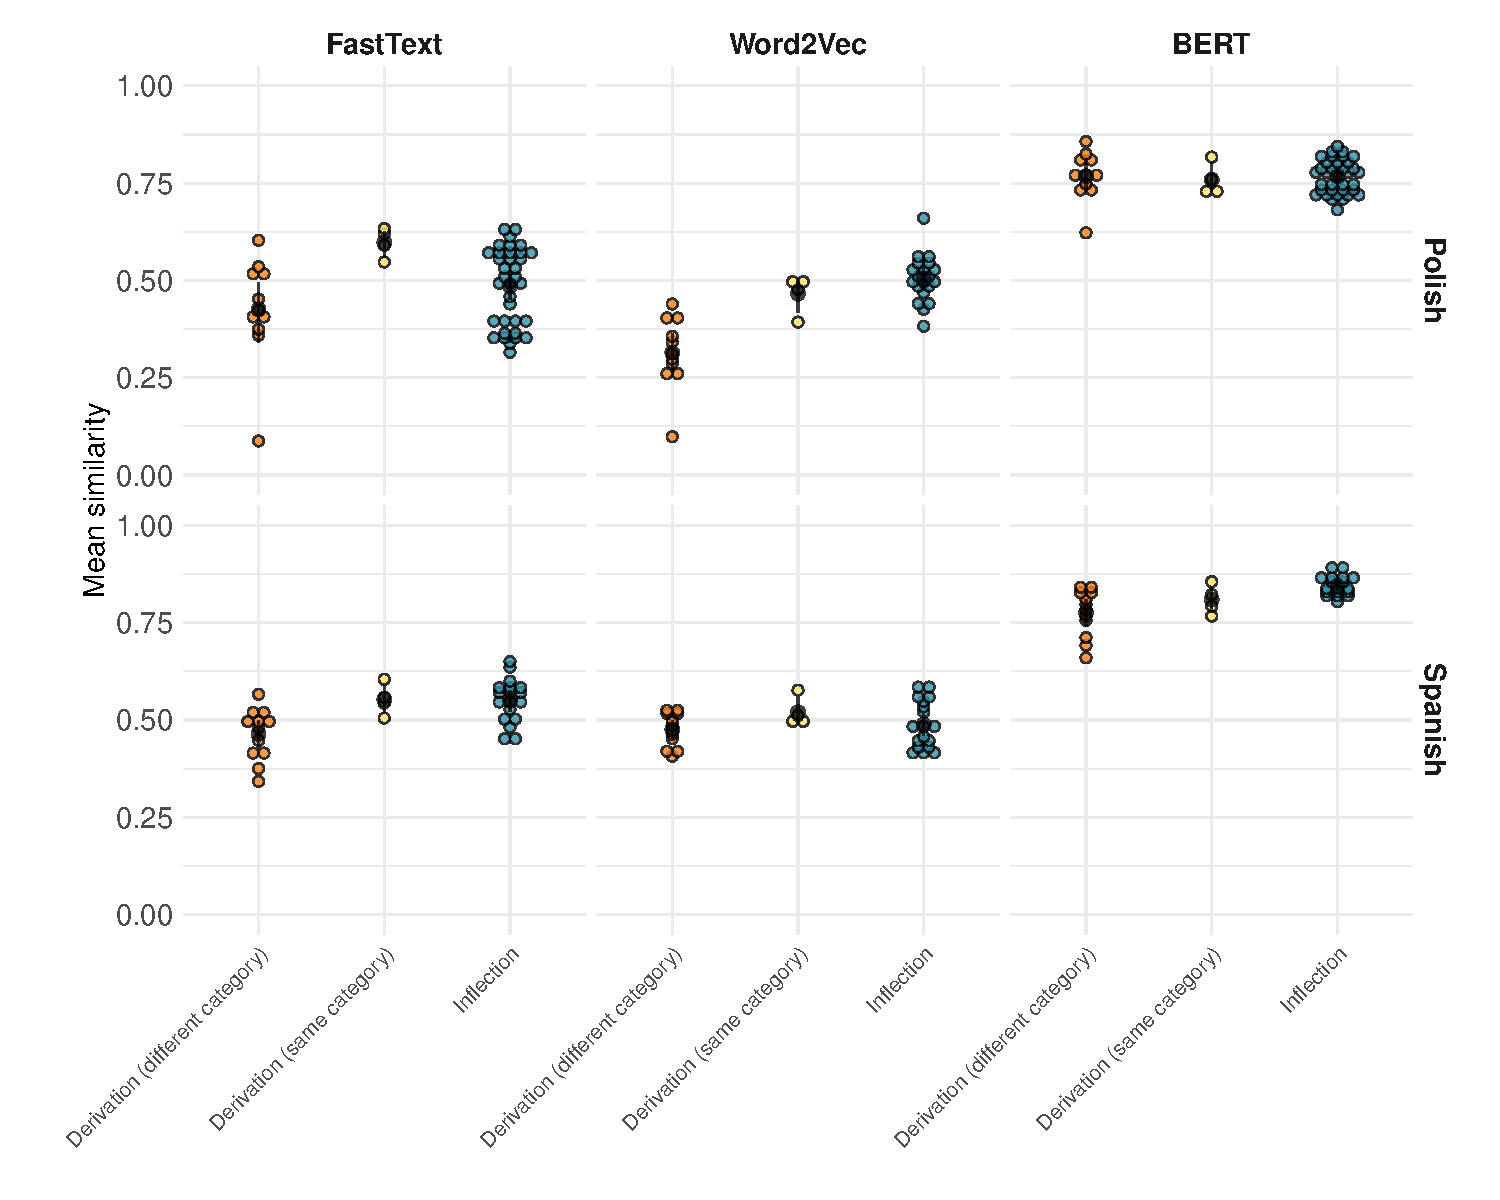
\includegraphics[width=\textwidth]{fig-clean.pdf}
\caption{Mean similarity between pivot and form in inflection and derivation by model and language. Each dot represents a category. The black dot represents the mean similarity of all the categories and the standard deviation around it.}
\label{fig:clean-data}
\end{figure}

\section{Discussion}

\section{Conclusion}

% Print bibliography
\newpage
\addcontentsline{toc}{section}{References}
\sloppy
\printbibliography

\end{document}
